\chapter{Introduction}

\textbf{Machine learning (ML)} is the study of computer algorithms that can improve automatically through experience and by the use of data. It is a branch of computer science which focuses on the use of data and algorithms to imitate the way that humans learn, graudally improving its accuracy\footnote{We will go much more in depth to the details of the term \textbf{accuracy} later.}.
Machine learning is an important component of the growing field of data science, through the use of statistical methods, machine learning algorithms build a model based on sample data, known as \emph{training data}, in order to make predictions or decisions without being explicitly programmed to do so.

Learning algorithms work on the basis that strategies, algorithms, and inferences that worked well in the past are likely to continue working well in the future. These inferences can be obvious, such as "since the sun rose every morning for the last 10,000 days, it will probably rise tomorrow morning as well". They can be nuanced, such as "\(X\%\) of families have geographically separate species with color variants, so there is a \(Y\%\) chance that undiscovered black swans exist".

Machine learning programs can perform tasks without being explicitly programmed to do so. It involves computers learning from data provided so that they carry out certain tasks. For simple tasks assigned to computers, it is possible to program algorithms telling the machine how to execute all steps required to solve the problem at hand; on the computer's part, no learning is needed. For more advanced tasks, it can be challenging for a human to manually create the needed algorithms. In practice, it can turn out to be more effective to help the machine develop its own algorithm, rather than having human programmers specify every needed step.

The discipline of machine learning employs various approaches to teach computers to accomplish tasks where no fully satisfactory algorithm is available. In cases where vast numbers of potential answers exist, one approach is to label some of the correct answers as valid. This can then be used as training data for the computer to improve the algorithm(s) it uses to determine correct answers. For example, to train a system for the task of digital character recognition, the MNIST dataset of handwritten digits has often been used.

Machine Learning allows computers to acquire \textbf{knowledge}. Knowledge is acquired through \textbf{algorithms} by learning and inferring from \textbf{data}, and it is presented by a \textbf{model} that is used on future data.

\section{When to use Machine Learning}
Machine learning algorithms are used in a wide variety of applications, such as in medicine, email filtering, speech recognition, and computer vision, where it is difficult or unfeasible to develop conventional algorithms to perform the needed tasks. It is important to remember that ML is not a solution for every type of problem. There are certain cases where robust solutions can be developed without using ML techniques. For example, you don't need ML if you can determine a target value by using simple rules, computations, or predetermined steps that can be programmed without needing any data-driven learning. In brief, Machine Learning can be involved in the following cases:
\setlist{nolistsep}
\begin{itemize}[topsep={0pt}, partopsep={0pt}]
    \item when human expertise does not exist;
    \item when humans cannot explain their expertise;
    \item when models must be customized;
    \item when models are based on huge amounts of data.
\end{itemize}

\subsubsection{When human expertise does not exist}
It may appear obvuois, when the human expertise lacks, then he cannot state to the machine the commands to execute. An examples is the Machine Learning techniques used for navigating to Mars: risk to human astronauts and interplanetary distance causing slow and limited communication drives scientists to pursue an autonomous approach to exploring distant planets, such as Mars. A portion of exploration of Mars has been conducted through the autonomous collection and analysis of Martian data by spacecraft such as the Mars rovers and the Mars Express Orbiter. The autonomy used on these Mars exploration spacecraft and on Earth to analyze data collected by these vehicles mainly consist of machine learning. 

\subsubsection{When humans cannot explain their expertise}
In this case it may be possible to have the necessary human expertise, but it is not possible to explain them to a machine. In order to make this more concrete, imagine that you need to do an algorithm that \emph{recognises} when a user says some words, it is very simple for a human to handle this job because there is a lot of human expertise, but it is infeasible to write a program (without Machine Learning) that can categorically recognise words. Speech recognition is a sub field of machine learning, and it involves various methodologies and technologies which allow recognising what the user is saying; while in voice recognition the machine learns to determine who is speaking.

\subsubsection{When models must be customized}
Sometimes we don't have a single solution, but we need to adapt the solution based to a moltitude variables. An example for this kind of problems is the personalized medicine. The purpose of personalized medicine is to select and deliver patient-specific treatments to achieve the best possible outcome. The challenge lies in identifying an optimum treatment as the number of possible predictors of good response like genetic and other biomarkers, and the option of treatments is increasing.

In addition to this, as most clinical trials are based upon average treatment effects, similar medicines become non-responsive for some patients and responsive for some other patients.

\subsubsection{When models are based on huge amounts of data}
As of 2021, 20 years have passed since the landmark completion of the draft human genome sequence. This milestone has led to the generation of an extraordinary amount of genomic data. Estimates predict that genomics research will generate between 2 and 40 exabytes of data within the next decade. DNA sequencing and other biological techniques will continue to increase the number and complexity of such data sets. This is why genomics researchers need AI/ML-based computational tools that can handle, extract and interpret the valuable information hidden within this large trove of data.

\begin{figure*}[b!]
  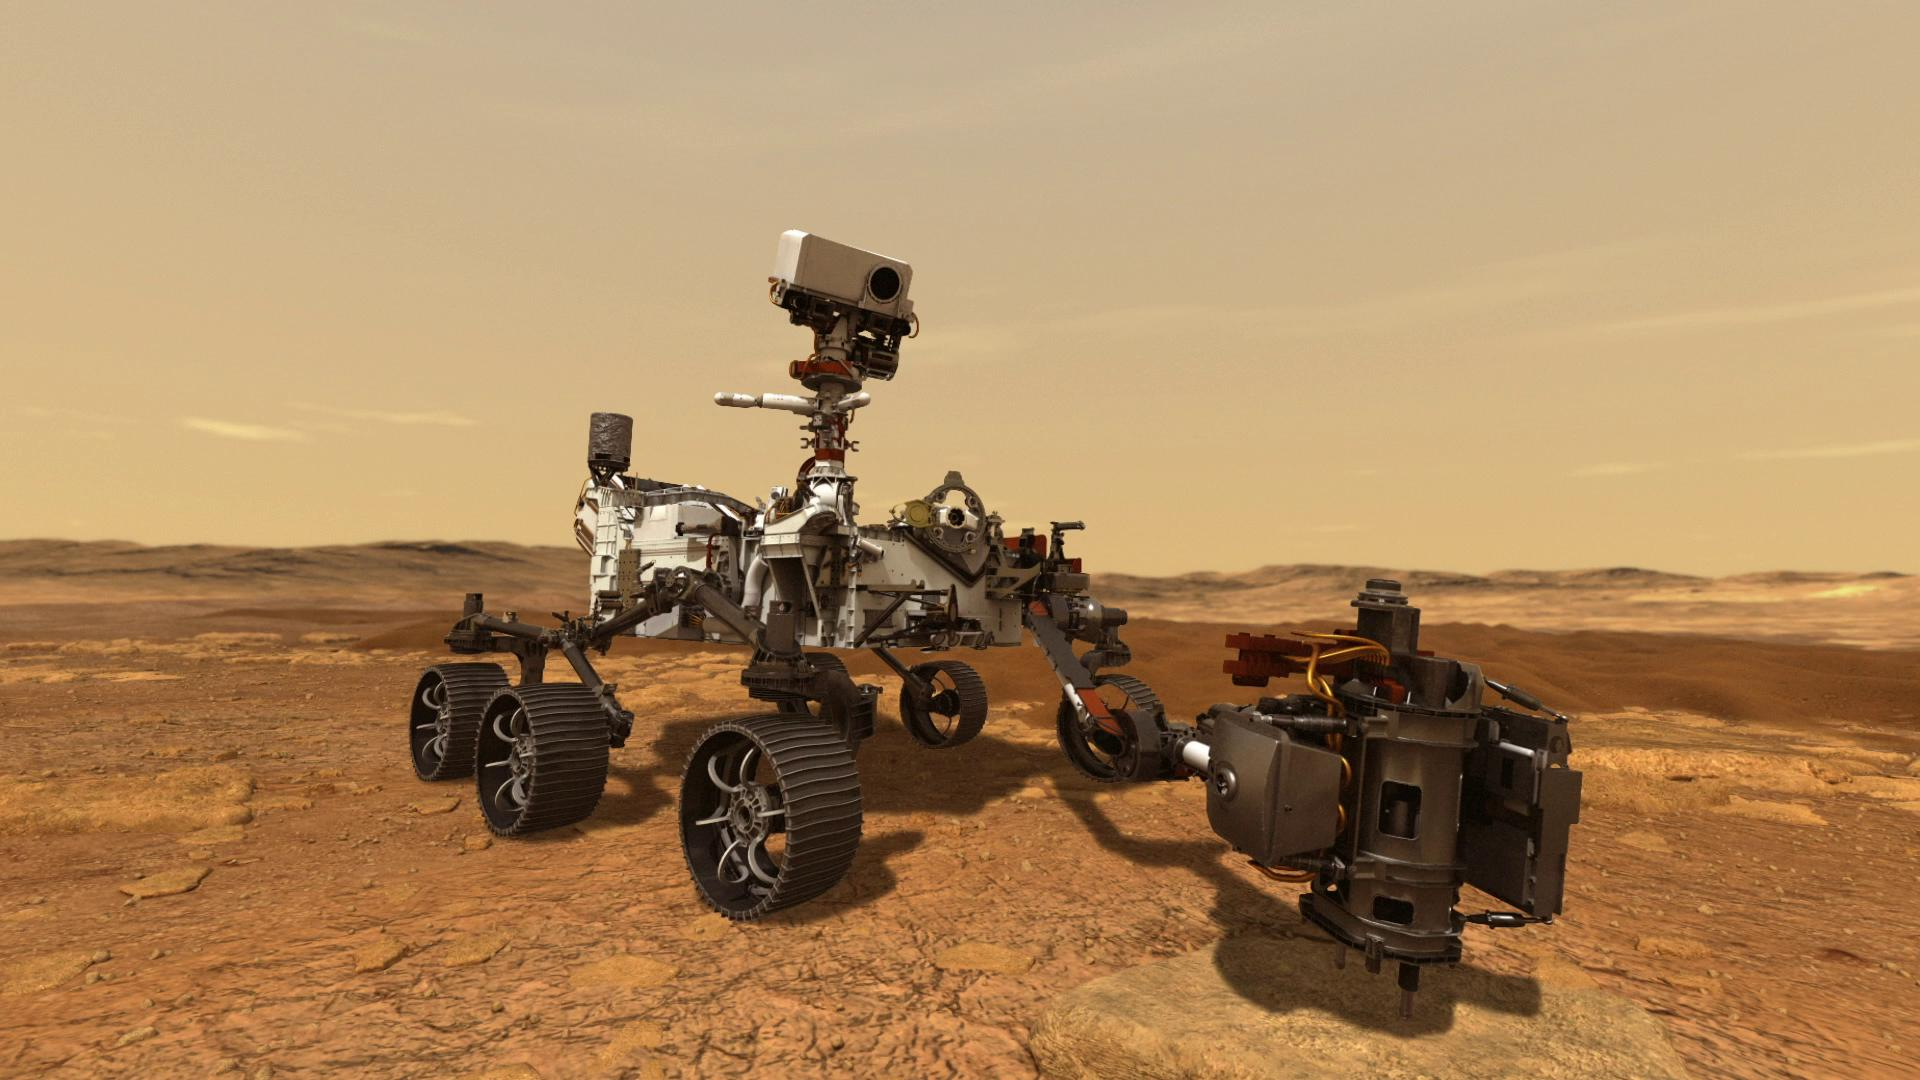
\includegraphics[width=.24\textwidth]{001a}\hfill
  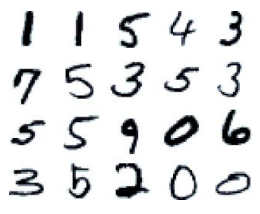
\includegraphics[width=.24\textwidth]{001b}\hfill
  
\includegraphics[width=.24\textwidth]{001c}\hfill
  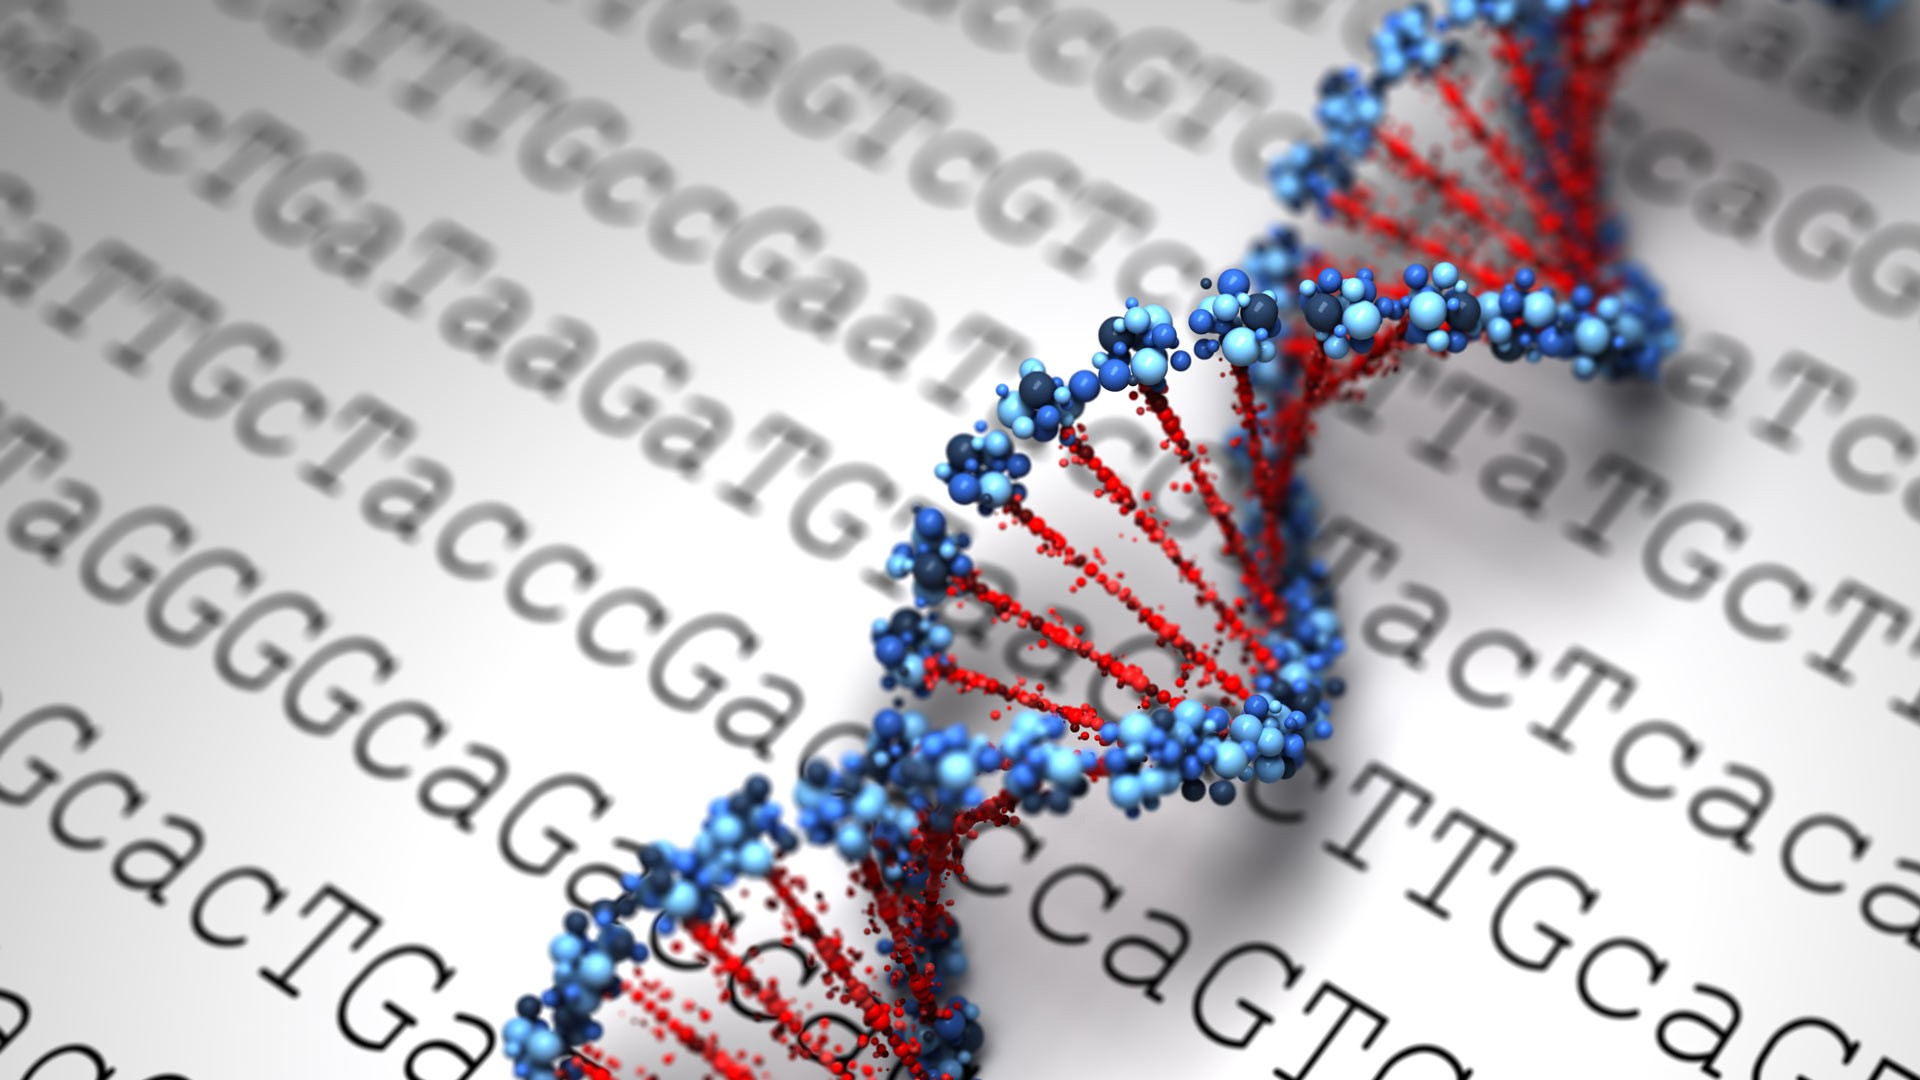
\includegraphics[width=.24\textwidth]{001d}
\end{figure*}

ML can be used for \textbf{recognizing} patterns, for example handwritten digits, facial and medical images; it can be used for \textbf{generating} patterns, for example for generating images or motion sequences; it can be used for recognizing anomalies, for example unusual credit card transactions or unusual patterns of sensor readings; or it can be used for \textbf{predictions}, for example it can be used to predict future stock prices or currency exchange rates, autonomous driving or to predict best moves in games.

\section{Definition}
Machine learning studies computer algorithms for learning to do stuff. We might, for instance, be interested in learning to complete a task, or to make accurate predictions, or to behave intelligently. The learning that is being done is always based on some sort of observations or data, such as examples, direct experience, or instruction. So in general, machine learning is about learning to do better in the future based on what was experienced in the past. Some more technical definitions have been provided during the development of machine learning:
\begin{itemize}[itemsep=.2em]
    \item It is concerned with the automatic discovery of regularities in data through the use of computer algorithms and with the use of these regularities to take actions. --- Chrisopher M. Bishop
    \item The goal of machine learning is to deveop methods that can automatically detect patterns in data, and then to use the uncovered patterns to predict future data or other outcomes of interest. --- Kevin P. Murphy
    \item Machine learning is about predicting the future based on the past. --- Hal Daume III
    \item A computer program is said to learn form \textbf{experience} \(E\) with resepct to some class of \textbf{tasks} \(T\) and performance \textbf{measure} \(P\), if its performance at tasks in \(T\), as measured by \(P\), improves with experience \(E\). --- T. Mitchell
\end{itemize}

\begin{figure}[t!]
  \begin{center}
  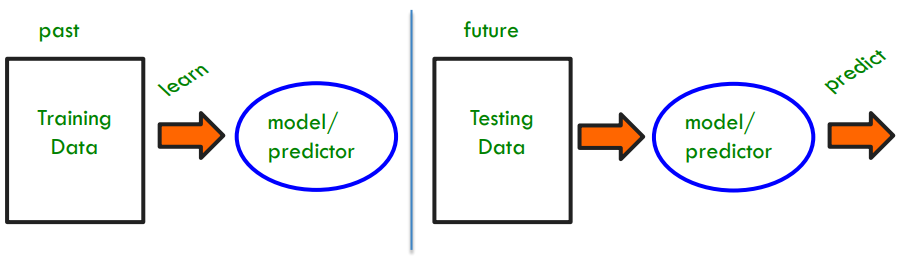
\includegraphics[width=0.75\textwidth]{002}
  \end{center}
\end{figure}

\subsection{Formally}
Mathematically speaking, machine learning is the study of algorithms that improve their performance \(P\) at some task \(T\) with experience \(E\). A well-defined learning task is given by a triplet \( \langle T,P,E \rangle \).

\begin{example}[Tasks for machine learning applications]
    For handwritten word recognition, the learning task \( \langle T,P,E \rangle \) is defined as follows:
    \begin{itemize}
        \item[T:] Recognizing handwritten words;
        \item[P:] Percentage of words correctly classified;
        \item[E:] Database of human-labeled images of handwritten words.
    \end{itemize}
    \tcblower
    For the spam email recognition, the learning task \( \langle T,P,E \rangle \) is defined as follows:
    \begin{itemize}
      \item[T:] Categorizing email messages as spam or legitimate;
      \item[P:] Percentage of email messages correctly classified;
      \item[E:] Database of emails, some with human-given labels.
    \end{itemize}
\end{example}

\section{Machine Learning vs Other Disciplines}
Modern day machine learning has two objectives, one is to classify data based on models which have been developed, the other purpose is to make predictions for future outcomes based on these models. A hypothetical algorithm specific to classifying data may use computer vision of moles coupled with supervised learning in order to train it to classify the cancerous moles. Where as, a machine learning algorithm for stock trading may inform the trader of future potential predictions.

\subsection{Artificial Intelligence}
\begin{wrapfigure}{r!}{0.35\textwidth}
    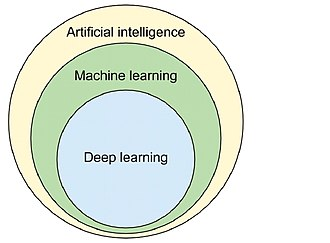
\includegraphics[width=0.35\textwidth]{003}
    \caption{Machine Learning as subfield of AI}
  \label{fig:003}
\end{wrapfigure}
Artificial intelligence (AI) is intelligence demonstrated by machines, as opposed to natural intelligence displayed by animals including humans. Leading AI textbooks define the field as the study of "intelligent agents": any system that perceives its environment and takes actions that maximize its chance of achieving its goals.

Some popular accounts use the term "artificial intelligence" to describe machines that mimic "cognitive" functions that humans associate with the human mind, such as "learning" and "problem solving", however, this definition is rejected by major AI researchers.

AI applications include advanced web search engines (e.g., Google), recommendation systems (used by YouTube, Amazon and Netflix), understanding human speech (such as Siri and Alexa), self-driving cars (e.g., Tesla), automated decision-making and competing at the highest level in strategic game systems (such as chess and Go). As machines become increasingly capable, tasks considered to require "intelligence" are often removed from the definition of AI, a phenomenon known as the AI effect. For instance, optical character recognition is frequently excluded from things considered to be AI, having become a routine technology.

\subsection{Deep Learning}
\begin{wrapfigure}{l!}{0.35\textwidth}
  \begin{center}
    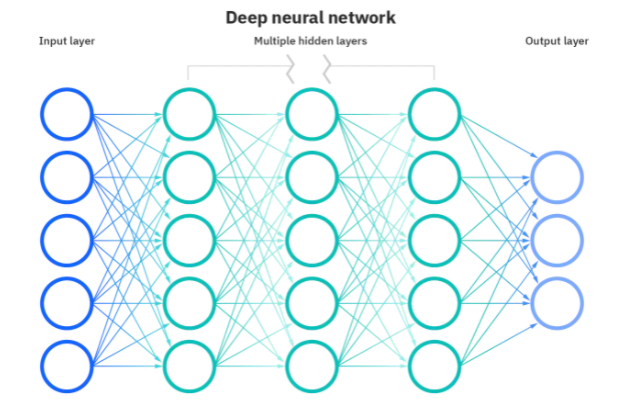
\includegraphics[width=0.35\textwidth]{004}
  \end{center}
  \label{fig:004}
\end{wrapfigure}
Deep Learning is part of a broader family of machine learning methods based on artificial neural networks with representation learning. Artificial neural networks (ANNs) were inspired by information processing and distributed communication nodes in biological systems. ANNs have various differences from biological brains. Specifically, artificial neural networks tend to be static and symbolic, while the biological brain of most living organisms is dynamic (plastic) and analogue.

The adjective "deep" in deep learning refers to the use of multiple layers in the network. Early work shows that a linear perceptron\footnote{\textbf{Perceptron:} is an algorithm for supervised learning of binary classifiers --- a function which can decide whether or not an input belongs to some specific class.} cannot be a universal classifier, but that a network with a nonpolynomial activation function with one hidden layer of unbounded width can. Deep learning is a modern variation which is concerned with an unbounded number of layers of bounded size, which permits pratical application and optimized implementation, while retaining theoretical universality under mild conditions. In deep learning the layers are also permitted to be heterogeneous and to deviate widely from biologically informed connectionist models, for the sake of efficiency, trainability and understandability, whence the "structured" part.

In deep learning, each level learns to transform its input data into a slightly more abstract and composite representation. In an image recognition application, the raw input may be a matrix of pixels; the first representational layer may abstract the pixels and encode edges; the second layer may compose and encode arrangements of edges; the third layer may encode a nose and eyes; and the fourth layer may recognize that the image contains a face. Importantly, a deep learning process can learn which features to optimally place in which level on its own. This does not eliminate the need for hand-tuning; for example, varying numbers of layers and layer sizes can provide different degrees of abstraction.

\subsection{Data Mining}
Data mining is a process of searching, extracting and analyzing (that may include) discovering various types of text graphic patterns (as calligraphic for example), language and literary figures, stylistics, in large amounts of textual or mixed visual and textual data sets, that also involvs methods at the intersection of machine learning, formal linguistics analyses as textual statistics, and database systems.

The actual data mining task is the semi-automatic or automatic analysis of large quantities of textual databases to extract previously not well known or entirely unknown, interesting or surprising language or information patterns such as groups of textual data records, but also unusual records (sometimes computer detected as anomaly), but also associations or dependencies (rule of pattern association and sequential pattern mining). This usually involves using database techniques such as using of spatial indices. These textual or information patterns can then be seen as summarizing of the input data, and may be used in further analysis or, for example, in machine learning for analysis involving predictions.

\section{Back to machine learning}

The general set up of predicting the future based on the past is at the core of most machine learning. The objects that our algorithm will make predictions about are \textbf{examples}. Let's consider for example the Netflix recommender system: when you watch a movie and state that you liked (or disliked) it, Netflix takes this as an example, and the like or dislike as a label that will make the algorithm learn from this example. 

\begin{wrapfigure}{r!}{0.35\textwidth}
  \begin{center}
    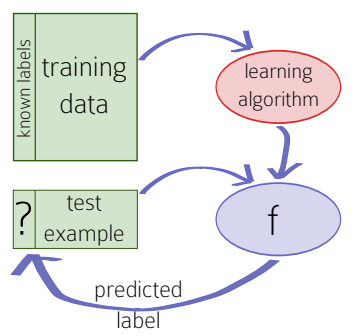
\includegraphics[width=0.35\textwidth]{005}
  \end{center}
  \caption{}
  \label{fig:005}
\end{wrapfigure}

To make this concrete, Figure~\ref{fig:005} shows the general framework of induction. We are given \textbf{training data} on which our algorithm is expected to learn. This training data is the examples that Alice observes, or the historical rating data for the recommender system. 
Based on this training data, our learning algorithm induces a function \(f\) that will map a new example to a corresponding prediction.

We want our algorithm to be able to make lots of predictions, so we refer to the collection of examples on which we will evaluate our algorithm as the \textbf{test set}. The test set is a closely guarded secret: it is the final exam on which our learning algorithm is being testes. 

The goal of inductive machine learning is to take some training data and use it to induce a function \(f\). This function \(f\) will be evaluated on the test data. The machine learning algorithm has succeeded if its performance on the test data is high.

\newpage
\begin{exercise}[topsep=20pt,itemsep=10pt]
  \ex When is Machine Learning recommended and when it is not? Give some example.
  \ex Give some example of Machine Learning algorithms on real applications.
  \ex Give the formal definition of Machine Learning and provide some example of task.
  \ex Provide the definition of Artificial Intelligence and Deep Learning enphasizing the differences from Machine Learning.
  \ex What are the examples?
  \ex How are the training data and the test data used?
\end{exercise}